\documentclass[10pt]{article}
\usepackage[utf8]{inputenc}
\usepackage[T1]{fontenc}
\usepackage{amsmath}
\usepackage{amsfonts}
\usepackage{amssymb}
\usepackage[version=4]{mhchem}
\usepackage{stmaryrd}
\usepackage{hyperref}
\hypersetup{colorlinks=true, linkcolor=blue, filecolor=magenta, urlcolor=cyan,}
\urlstyle{same}
\usepackage{graphicx}
\usepackage[export]{adjustbox}
\graphicspath{ {./images/} }
\usepackage{caption}

\title{Assistance of metal nanoparticles in photocatalysis - nothing more than a classical heat source }

\author{Yonatan Sivan, (ID*ad leng Wai Un ${ }^{\text {abd }}$ and Yonatan Dubi ${ }^{\text {cd }}$}
\date{}


%New command to display footnote whose markers will always be hidden
\let\svthefootnote\thefootnote
\newcommand\blfootnotetext[1]{%
  \let\thefootnote\relax\footnote{#1}%
  \addtocounter{footnote}{-1}%
  \let\thefootnote\svthefootnote%
}

%Overriding the \footnotetext command to hide the marker if its value is `0`
\let\svfootnotetext\footnotetext
\renewcommand\footnotetext[2][?]{%
  \if\relax#1\relax%
    \ifnum\value{footnote}=0\blfootnotetext{#2}\else\svfootnotetext{#2}\fi%
  \else%
    \if?#1\ifnum\value{footnote}=0\blfootnotetext{#2}\else\svfootnotetext{#2}\fi%
    \else\svfootnotetext[#1]{#2}\fi%
  \fi
}

\begin{document}
\maketitle
\captionsetup{singlelinecheck=false}
Received 4th October 2018, Accepted 2nd November 2018\\
DOI: 10.1039/c8fd00147b

\begin{abstract}
In a recent paper, we derived a self-consistent theory of the steady-state electron distribution of a metal under continuous wave illumination which treats thermal and non-thermal effects on the same footing. Here, we re-derive the main analytical results of that study from very simple arguments, and draw a series of conclusions which contradict claims made in previous studies of the steady-state distribution. In particular, we show that the faster chemical reactions reported in many previous papers are extremely unlikely to originate from high energy non-thermal electrons. Instead, the faster reactions very likely originate from a purely thermal effect.
\end{abstract}

\section*{I. Introduction}
In recent years, a central focus of research into nanoplasmonics has been on finding ways to exploit the enhanced absorption exhibited by nanoplasmonic systems. Two main routes are discussed in the literature. First, it was shown that plasmonic nanostructures can be efficient sources of heat on the nanoscale, ${ }^{\mathbf{1 , 2}}$ a research topic that is usually referred to as thermo-plasmonics. This has enabled a wide range of emerging applications at different temperature ranges, such as photothermal imaging, ${ }^{3,4}$ cancer treatment, ${ }^{5}$ plasmonic photovoltaics, ${ }^{6}$ water boiling, sanitation and super-heating, ${ }^{7-9}$ solvothermal (hydro-thermal) chemistry, ${ }^{\mathbf{1 0}}$ thermo-photovoltaics, ${ }^{\mathbf{1 1 , 1 2}}$ diffusive switching, ${ }^{\mathbf{1 3}}$ thermoelectrics, ${ }^{\mathbf{1 4}}$ plasmon-assisted chemical vapor deposition ${ }^{15}$ and heat-assisted magnetic recording, ${ }^{\mathbf{1 6}}$ which may involve temperatures even higher than 2000 K .

Clearly, the generation of heat is a result of internal thermalization processes that convert the high energy non-thermal electron distribution generated initially by the absorption of photons to a thermal distribution. In that context, a second way to exploit heat has emerged - it was hypothesized that the initially generated

\footnotetext{${ }^{a}$ Unit of Electro-Optics Engineering, Ben-Gurion University, Israel. E-mail: \href{mailto:sivanyon@bgu.ac.il}{sivanyon@bgu.ac.il}\\
${ }^{b}$ Joan and Irwin Jacobs TIX Institute, National Tsing Hua University, Taiwan\\
${ }^{\text {c }}$ Department of Chemistry, Ben-Gurion University, Israel\\
${ }^{\text {d }}$ Ilse Katz Center for Nanoscale Science and Technology, Ben-Gurion University, Israel
}
high energy non-thermal (frequently (ill-)referred to as "hot") electrons could be used as a means to catalyze photochemical reactions, ${ }^{\mathbf{1 7 - 2 3}}$ as well as in artificial photosynthesis, ${ }^{\mathbf{2 4 , 2 5}}$ photo-detection, ${ }^{\mathbf{2 6 - 3 0}}$ frequency upconversion ${ }^{\mathbf{3 1 , 3 2}}$ etc. Specifi- cally, a large number of experimental studies have reported faster chemical reactions in the presence of illuminated metal nanoparticles. ${ }^{\mathbf{1 9 , 2 0 , 3 3}}$ However, it was not clear whether this acceleration of chemical reactions occurred due to the increased population of high energy carriers, or due to the mere (consequent) increase in temperature; in other words - is it thermal or non-thermal effects that are responsible for the faster chemistry? This is important to know because although heating is frequently used in catalysis, it is accompanied by various undesired side effects (such as the enhancement of additional parasitic reactions) ${ }^{\mathbf{1 8}}$ and incurs significant practical and financial complications for real-life applications. As a result, heating is generally avoided in practice.

Very few attempts have been made to distinguish experimentally between thermal and non-thermal effects. This should be done by reproducing the same temperature rise caused by laser illumination through the use of purely external heating. Clearly, it is very difficult to measure temperature on the nanoscale with sufficient spatial resolution; indeed, thermometry methods for metal nanostructures have emerged only in the last few years (e.g. ref. 34-36). An alternative determination of the temperature via numerical simulation is simple for a single nanoparticle (NP), ${ }^{37,38}$ but non-trivial in the presence of many nanoparticles due to the long range inter-particle thermal interactions ${ }^{\mathbf{3 9 , 4 0}}$ which give rise to (highly) non-uniform temperatures on multiple length-scales. For example, in ref. 41 the control experiment showed that the chemistry is sensitive to the external temperature, i.e. the metal does more than just enhance photon absorption. ${ }^{42}$ However, the control experiment was carried out at a temperature measured far away from the illuminated nanoparticles, and this was most likely lower than the actual nanoparticle temperature, as noted later on by the same group of authors ${ }^{\mathbf{4 3}}$ and by others. ${ }^{44}$ Even if the temperature is known, it is not easy to perform meaningful control experiments due to the difficulty in reproducing the nonuniform temperature distribution across the typical suspension volume with an external heat source. In pulsed experiments, this is even more difficult due to the transient nature of the temperatures and the differences between the electron and lattice temperatures.

In addition to all these practical complications, there has been also a fundamental controversy regarding the definition of temperature for metal nanostructures under illumination. Indeed, one could naively argue that upon illumination, the system is out of equilibrium, meaning that temperature inherently an equilibrium property - cannot be well defined. ${ }^{45}$ Accordingly, while temperatures were defined after the initial non-equilibrium stage that follows ultrafast illumination (see for example ref. 46 and 47), all previous theoretical studies of continuous wave (CW) illumination treated the non-equilibrium in great detail, but ignored the possibility of an increase in the electron and phonon temperatures to above the environment temperature.

In order to reconcile this paradox, in ref. 48 we suggested a unique solution for the determination of the steady-state temperature developing in a metal nanostructure, based only on energy conservation and basic thermodynamics. Specifically, we developed a self-contained theory for the photo-generation of nonthermal energetic carriers in metal nanostructures based on a quantum-like\\
version of the Boltzmann equation (BE). $\mathbf{4 , 4 7 , 4 9 - 5 7}^{\mathbf{4 7}}$ To the BE we added, in a selfconsistent way, electron-phonon scattering and energy leakage to the environment via phonon-phonon coupling, such that the electron and phonon (lattice) temperatures in the plasmonic nanostructure can rise above the ambient temperature. The steady-state solution of this set of equations ensures energy conservation - the power flowing into the metal due to photon absorption is exactly balanced by heat leakage to the environment. Since there is obviously only one pair of values for the electron and phonon temperatures for which this happens, the approach of ref. 48 enables a determination of the temperature(s) of a system which is out of equilibrium in a unique and unambiguous way. This approach also enables a comparison, for the first time to our knowledge, of the relative importance of thermal and non-thermal effects.

The simulations showed that the population of non-thermal energetic electrons and holes ${ }^{88}$ can increase dramatically under illumination, yet this process is extremely inefficient, as the majority of the absorbed energy leads to heating; the electron and phonon temperatures are found to be similar, thus justifying the use of the (classical) single temperate heat model. ${ }^{2}$ Somewhat surprisingly, we found that just above (below) the Fermi energy, the non-equilibrium consists of holes (electrons), rather than the other way around; we showed that this behaviour is due to the dominance of e-ph collisions.

The results of ref. 48 were based on a rather complicated and slowly converging numerical procedure involving standard but cumbersome scattering integrals. This approach also lacks deep physical insights. In the current manuscript, we provide several simple estimates of the numerical results obtained in ref. 48 that partially obviate the need for the heavy/lengthy numerical procedure performed so far. We also apply the results of ref. 48 to show that, unlike what is frequently claimed in the literature, the density of high energy non-thermal carriers is, to leading order at least, independent of the NP size and shape, and that in fact, small spherical NPs are the least efficient source of high energy non-thermal carriers. Furthermore, we develop a simple model for photocatalysis which shows that it is highly unlikely that the faster chemical reactions observed experimentally are due to the generation of non-thermal, high energy carriers in the metal. The faster reactions much more likely originate from a purely thermal effect. Finally, we describe several experiments that have to be carried out to confirm our predictions.

\section*{II. A simple calculation of the electron distribution and temperatures}
In this section, we briefly reintroduce the theoretical model reported in ref. 48 and show how to obtain some of its numerical results without going though a fullscale numerical calculation, based on standard, physically-sensible assumptions.

The Boltzmann equation (BE) is


\begin{equation*}
\frac{\partial f(\mathcal{E}) ; T_{\mathrm{e}}, T_{\mathrm{ph}}}{\partial t}=\underbrace{\left(\frac{\partial f}{\partial t}\right)}_{\text {photon absorption }}+\underbrace{\left(\frac{\partial f}{\partial t}\right)}_{\text {e-e collisions }}+\underbrace{\left(\frac{\partial f}{\partial t}\right)}_{\text {e-ph collisions }} . \tag{1}
\end{equation*}


Here, $f$ is the electron distribution function at an energy, $\mathcal{E}$, electron temperature, $T_{\mathrm{e}}$ and phonon temperature, $T_{\mathrm{ph}}$, representing the population probability of\\
electrons in a system characterized by a continuum of states within the conduction band. The first term on the right-hand-side (RHS) of eqn (1) describes the excitation of conduction electrons due to photon absorption (see Appendix: A for its explicit form). The second term on the RHS of eqn (1) describes the energy relaxation due to collisions between electrons and phonons (see ref. 48 and 54 for its explicit form). The third term on the RHS of eqn (1) represents the thermalization induced by e-e collisions, i.e. the convergence of the non-thermal population into the thermalized Fermi-Dirac distribution, given by


\begin{equation*}
f^{\mathrm{T}}\left(\mathcal{E} ; T_{\mathrm{e}}\right)=\left(1+\mathrm{e}^{\left(\mathcal{E}-\mathcal{E}_{\mathrm{F}}\right) / k_{\mathrm{B}} T_{\mathrm{e}}}\right)^{-1} . \tag{2}
\end{equation*}


Here, $k_{\mathrm{B}}$ is the Boltzmann constant and $\mathcal{E}_{\mathrm{F}}$ is the Fermi energy. ${ }^{89}$ The explicit form of the e-e relaxation term used in our formulation can be found in ref. 48. Note that eqn (1) does not account for interband transitions. In that sense, it is suitable for describing Ag NPs, but is relatively less accurate for Au NPs. See ref. 47 and 48 for a detailed justification of this model.

We now split the electron distribution into a thermal and non-thermal part, namely, we define $\Delta f^{\mathrm{NT}} \equiv f\left(\mathcal{E}, T_{\mathrm{e}}, T_{\mathrm{ph}}\right)-f^{\mathrm{T}}\left(\mathcal{E}, T_{\mathrm{e}}\right)$ in ref. 48 . We then multiply the resulting equations by the product of the electron energy, $\mathcal{E}$, and the density of electron states, $\rho_{\mathrm{e}}(\mathcal{E})$, and integrate over the electron energy. The resulting equations describe the dynamics of the 3 energy channels, namely, non-thermal electron energy, thermal energy and phonon energy:

$$
\begin{gathered}
\frac{\mathrm{d} \mathcal{U}_{\mathrm{e}}^{\mathrm{NT}}}{\mathrm{~d} t}=-W_{\mathrm{e}-\mathrm{e}}-W_{\mathrm{e}-\mathrm{ph}}^{\mathrm{NT}}+W_{\mathrm{ex}}^{\mathrm{NT}} \\
\frac{\mathrm{~d} \mathcal{U}_{\mathrm{e}}^{\mathrm{T}}}{\mathrm{~d} t}=W_{\mathrm{e}-\mathrm{e}}-W_{\mathrm{e}-\mathrm{ph}}^{\mathrm{T}}+W_{\mathrm{ex}}^{\mathrm{T}} \\
\frac{\mathrm{~d} \mathcal{U}_{\mathrm{ph}}^{\mathrm{T}}}{\mathrm{~d} t}=W_{\mathrm{e}-\mathrm{ph}}^{\mathrm{T}}+W_{\mathrm{ph}-\mathrm{env}}+W_{\mathrm{e}-\mathrm{ph}}^{\mathrm{NT}}
\end{gathered}
$$

Here, $\mathcal{U}_{\mathrm{e}}^{\mathrm{NT}}=\int \mathcal{E} \rho_{\mathrm{e}}(\mathcal{E})\left[f-f^{\mathrm{T}}\right] \mathrm{d} \mathcal{E}$ is the total energy of the non-thermal electron sub-system, and we define the energy change rates due to photo-excitation $\left(W_{\mathrm{ex}}^{\mathrm{NT}} \equiv \int \mathcal{E} \rho_{\mathrm{e}}(\mathcal{E})\left[\left(\frac{\mathrm{d} f}{\mathrm{~d} t}\right)_{\mathrm{ex}}-\left(\frac{\mathrm{d} f^{\mathrm{T}}}{\mathrm{d} t}\right)_{\mathrm{ex}}\right] \mathrm{d} \mathcal{E}\right.$ and $\left.W_{\mathrm{ex}}^{\mathrm{T}} \equiv \int \mathcal{E} \rho_{\mathrm{e}}(\mathcal{E})\left(\frac{\mathrm{d} f^{\mathrm{T}}}{\mathrm{d} t}\right)_{\mathrm{ex}} \mathrm{d} \mathcal{E}\right), \quad \mathrm{e}-\mathrm{e}$\\
collisions $\left(W_{\mathrm{e}-\mathrm{e}} \equiv \int \mathcal{E} \rho_{\mathrm{e}}(\mathcal{E})\left(\frac{\partial f}{\partial t}\right)_{\mathrm{e}-\mathrm{e}} \mathrm{d} \mathcal{E}\right), \mathrm{e}-\mathrm{ph}$ collisions $\left(W_{\mathrm{e}-\mathrm{ph}}^{\mathrm{NT}} \equiv-\int \mathcal{E} \rho_{\mathrm{e}}(\mathcal{E})\right.$\\
$\left[\left(\frac{\partial f}{\partial t}\right)_{\mathrm{e}-\mathrm{ph}}-\left(\frac{\partial f^{\mathrm{T}}}{\partial t}\right)_{\mathrm{e}-\mathrm{ph}}\right] \mathrm{d} \mathcal{E}$ and $\left.W_{\mathrm{e}-\mathrm{ph}}^{\mathrm{T}} \equiv-\int \mathcal{E} \rho_{\mathrm{e}}(\mathcal{E})\left(\frac{\partial f^{\mathrm{T}}}{\partial t}\right)_{\mathrm{e}-\mathrm{ph}} \mathrm{d} \mathcal{E}\right), \quad$ and the coupling of energy to the environment ( $W_{\text {ph-env }}$ ).

\section*{A. Determining the steady-state temperatures}
We now show how the steady-state electron and phonon temperatures can be determined without the need for the lengthy exact numerical calculations of the Boltzmann equation.

In order to avoid the heavy numerical computation of the BE and the rate equations above, we adopt several standard approximations. First, we approximate $W_{\mathrm{e}-\mathrm{e}}$ and $W_{\mathrm{e}-\mathrm{ph}}^{\mathrm{NT}}$ as $\Gamma_{\mathrm{e}} \mathcal{U}_{\mathrm{e}}^{\mathrm{NT}}$ and $\Gamma_{\mathrm{ph}} \mathcal{U}_{\mathrm{e}}^{\mathrm{NT}}$, where $\Gamma_{\mathrm{e}}$ and $\Gamma_{\mathrm{ph}}$ are the effective time scales that represent the decay of the non-thermal energy due to e-e and e-ph collisions, respectively. Such an estimate is customary within the approach known as the (extended) Two Temperature Model ((e)TTM), initially introduced phenomenologically ${ }^{\mathbf{5 8}}$ and later derived from a classical point of view in ref. 59. As an initial guess, we can set $\Gamma_{\mathrm{e}}^{-1} \sim 0.5 \mathrm{ps}$ and $\Gamma_{\mathrm{ph}}^{-1} \sim 1 \mathrm{ps} .^{\mathbf{5 3 , 5 8 - 6 0}}$ We also replace $W_{\mathrm{e}-\mathrm{ph}}^{\mathrm{T}}$ with $G_{\mathrm{e}-\mathrm{ph}}\left(T_{\mathrm{e}}-T_{\mathrm{ph}}\right)$, an approximation which has been shown to be an excellent approximation for $T_{\mathrm{e}}<3000 \mathrm{~K} .^{\mathbf{4 6 , 5 4 , 6 1 - 6 3}}$ Following this, the above rate equations become

$$
\begin{gathered}
\frac{\mathrm{d} \mathcal{U}_{\mathrm{e}}^{\mathrm{NT}}}{\mathrm{~d} t}=-\Gamma_{\mathrm{e}} \mathcal{U}_{\mathrm{e}}^{\mathrm{NT}}-\Gamma_{\mathrm{ph}} \mathcal{U}_{\mathrm{e}}^{\mathrm{NT}}+W_{\mathrm{ex}}^{\mathrm{NT}}, \\
\frac{\mathrm{~d} \mathcal{U}_{\mathrm{e}}^{T}}{\mathrm{~d} t}=\Gamma_{\mathrm{e}} \mathcal{U}_{\mathrm{e}}^{\mathrm{NT}}-G_{\mathrm{e}-\mathrm{ph}}\left(T_{\mathrm{e}}-T_{\mathrm{ph}}\right)+W_{\mathrm{ex}}^{T}, \\
\frac{\mathrm{~d} \mathcal{U}_{\mathrm{ph}}}{\mathrm{~d} t}=G_{\mathrm{e}-\mathrm{ph}}\left(T_{\mathrm{e}}-T_{\mathrm{ph}}\right)-G_{\mathrm{ph}-\mathrm{env}}\left(T_{\mathrm{ph}}-T_{\mathrm{env}}\right)+\Gamma_{\mathrm{ph}} \mathcal{U}_{\mathrm{e}}^{\mathrm{NT}},
\end{gathered}
$$

where we also set $W_{\text {ph-env }}=G_{\text {ph-env }}\left(T_{\text {ph }}-T_{\text {env }}\right)$. This set of equations in fact provides a self-consistent derivation of the (e)TTM from the BE; similar derivations were previously suggested in ref. 64-66, 90 and 91.

For CW illumination, the system is in a steady-state. Thus, $\mathcal{U}_{\mathrm{e}}^{\mathrm{NT}}=W_{\mathrm{ex}}^{\mathrm{NT}} /\left(\Gamma_{\mathrm{e}}+\Gamma_{\mathrm{ph}}\right)$,

$$
\frac{\Gamma_{\mathrm{e}}}{\Gamma_{\mathrm{e}}+\Gamma_{\mathrm{ph}}} W_{\mathrm{ex}}^{\mathrm{NT}}+W_{\mathrm{ex}}^{\mathrm{T}}=G_{\mathrm{e}-\mathrm{ph}}\left(T_{\mathrm{e}}-T_{\mathrm{ph}}\right)
$$

and

$$
G_{\mathrm{e}-\mathrm{ph}}\left(T_{\mathrm{e}}-T_{\mathrm{ph}}\right)=G_{\mathrm{ph}-\mathrm{env}}\left(T_{\mathrm{ph}}-T_{\mathrm{env}}\right)-\frac{\Gamma_{\mathrm{ph}}}{\Gamma_{\mathrm{e}}+\Gamma_{\mathrm{ph}}} W_{\mathrm{ex}}^{\mathrm{NT}}
$$

Therefore, via simple algebra, we can derive the following equations:


\begin{gather*}
T_{\mathrm{e}}=T_{\mathrm{ph}}+\frac{\frac{\Gamma_{\mathrm{e}}}{\Gamma_{\mathrm{e}}+\Gamma_{\mathrm{ph}}} W_{\mathrm{ex}}^{\mathrm{NT}}+W_{\mathrm{ex}}^{\mathrm{T}}}{G_{\mathrm{e}-\mathrm{ph}}}  \tag{3}\\
T_{\mathrm{ph}}=T_{\mathrm{env}}+\frac{W_{\mathrm{ex}}^{\mathrm{NT}}+W_{\mathrm{ex}}^{\mathrm{T}}}{G_{\mathrm{ph}-\mathrm{env}}} \tag{4}
\end{gather*}


Eqn (3) and (4) show that $T_{\mathrm{e}}$ and $T_{\mathrm{ph}}$ grow linearly with the incident intensity (via the absorbed power density, eqn (A1)-(A6)). The difference between the temperatures is also proportional to the absorbed power density. Most importantly, the difference between the two temperatures is independent of the particle size and coupling to the environment; it instead depends only on\\
the internal details of the electron subsystem and on the e-ph coupling coefficient, $G_{\mathrm{e}-\mathrm{ph}}$.

\section*{B. High energy non-thermal carrier density}
In order to determine the density of high energy non-thermal carriers, we exploit the fact that e-ph interactions are important only near the Fermi energy (see specifically ref. 48, Fig. S2(b)). The reason for that, by the FLT, is that the energy lost by a high energy non-thermal electron in a collision is a significant part of its excess energy with respect to the Fermi energy. Since that energy is much higher than the phonon energies, they are not generated during collisions of high energy non-thermal electrons. Thus, the electron population far away from the Fermi energy can be determined simply by balancing the electron excitation rate with the e-e collision rate. Indeed, we show in Appendix: A that the density of high energy non-thermal carriers is given by


\begin{equation*}
\Delta f^{\mathrm{NT}}(\mathcal{E}) \sim \tau_{\mathrm{e}-\mathrm{e}}(\mathcal{E}) R|E|^{2}, \tag{5}
\end{equation*}


where $R \equiv \frac{4 \varepsilon_{0} \varepsilon_{\mathrm{m}}^{\prime \prime}\left(\omega_{\mathrm{p}}\right)}{\hbar} \frac{\mathcal{E}_{\mathrm{F}}}{3 \mathcal{E}_{\max } n_{\mathrm{e}}}$ (definitions of the various parameters can be found in Appendix: A) and $E$ is the local electric field. This is found to be in excellent agreement with the numerical results (see Fig. 1).

Eqn (5) not only provides a simple way to compute the high energy, nonthermal carrier population, but also provides fundamental insight into the physics of non-thermal carrier generation. Specifically, it shows that the nonthermal carrier population is independent of the ambient temperature, phonon temperature and the temperature of the electrons, as well as of the thermal properties of the system. This means that previous studies of the steady-state electron distribution (e.g. ref. 67-70) could have been used to calculate quantitatively the high energy non-thermal carrier density correctly. ${ }^{92}$ However, they could not have been used to obtain the distribution near the Fermi energy because of the neglect of the temperature rise; accordingly, the relative amount of power going to the thermal and non-thermal channels has not been evaluated thus far. This also means that previous approaches incorrectly account for the role of interband transitions which, due to the need to bridge the bandgap energy, cause an increase in the non-thermal carrier distribution relatively close to the

\begin{figure}[h]
\begin{center}
  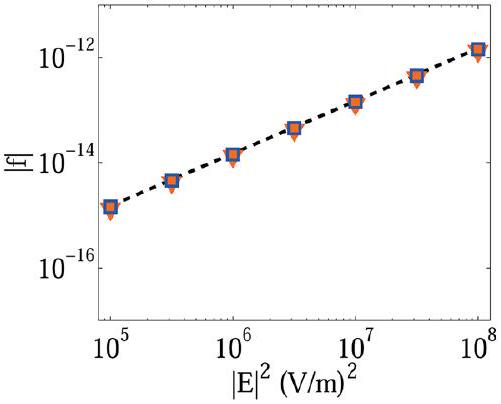
\includegraphics[alt={},max width=\textwidth]{9dd9846f-eb13-4506-8661-d691c4a998fa-06_404_501_1600_518}
\captionsetup{labelformat=empty}
\caption{Fig. 1 The population $f(\mathcal{E})$ of holes at $\mathcal{E}=1.8 \mathrm{eV}\left(<\hbar \omega_{\mathrm{p}}\right)$ below the Fermi level (blue rectangles) and electrons at $\mathcal{E}=1.8 \mathrm{eV}$ above the Fermi level (orange triangles), compared with the estimate (5) (black dashed line).}
\end{center}
\end{figure}

Fermi energy. ${ }^{68}$ In fact, assuming that the number of excess electrons generated near the Fermi energy is comparable to that in the high energy shoulders, it is most likely that their contribution would be negligible with respect to the thermal changes. Accordingly, one should re-examine all claims about the relative importance of interband transitions for the generation of non-thermal carriers. ${ }^{\mathbf{7 1}}$

A further implication of the accuracy of the estimate (5) is the independence of the density of high energy non-thermal carriers on the shape and size of the metal nanoparticle. Indeed, since it has been shown via fully quantum mechanical calculations that the e-e collision rates are independent of the particle size (e.g. ref. 47 and 72), it follows from eqn (5) that the density depends on the NP size and shape only via the value of the local field. This claim is corroborated by the numerical results of Section III below \& Fig. 2. This result is in contradiction to the claims that have frequently appeared in previous studies. It should be noted that the metal interface may support long-lived surface states which, in turn, might allow for a higher density of high energy non-thermal carriers. However, the importance of such states should be weighted by their relative number, which is surely small, especially for spherical nanoparticles of more than a few nm in size.

Finally, we note that the estimate (5) is essentially identical to the result for the population of the excited state in a system with discrete energy states (e.g. a two level system) in the weak excitation limit. This means that $\left(\tau_{\mathrm{e}-\mathrm{e}} R\right)^{-1 / 2}$ is essentially the effective saturation field for the metal, $\left|E_{\text {sat }}\right|=\sqrt{\mathrm{ZI}_{\text {sat }} /(2 n)} .^{\mathbf{9 3}}$ Then, assuming that the absorptivity of a single metal atom is comparable to that of a single gas atom or a semiconductor atom, it follows that since the relaxation rate of the metal electron is about 6 orders of magnitude faster compared with the relaxation of a gas or semiconductor atom, then the square of the saturation field, $\left|E_{\text {sat }}\right|^{2}$, of the metal will be 6 orders of magnitude higher than in an atomic gas or a semiconductor. For $I_{\text {sat }} \sim 10^{7} \mathrm{~W} \mathrm{~cm}^{-2}$ (typical for a gas or semiconductor atom), it is easy to see that $\left|E_{\text {sat }}\right|^{2} \sim 100 \Omega \cdot 10^{7} \mathrm{~W} \mathrm{~cm}^{-2}=10^{13} \mathrm{~V}^{2} \mathrm{~m}^{-2}$. In Appendix: A, we obtained $\left|E_{\text {sat }}\right|^{2} \sim 2.5 \times 10^{19} \mathrm{~V}^{2} \mathrm{~m}^{-2}$, which is in excellent agreement with the above estimate.

This shows that accounting for the discreteness of the energy states (as for the atomic physics case) or neglecting it (as in our approach) has, at most, a minor effect on the resulting density of high energy electrons. This conclusion is the opposite of the conclusions drawn in previous studies.

\begin{figure}[h]
\begin{center}
  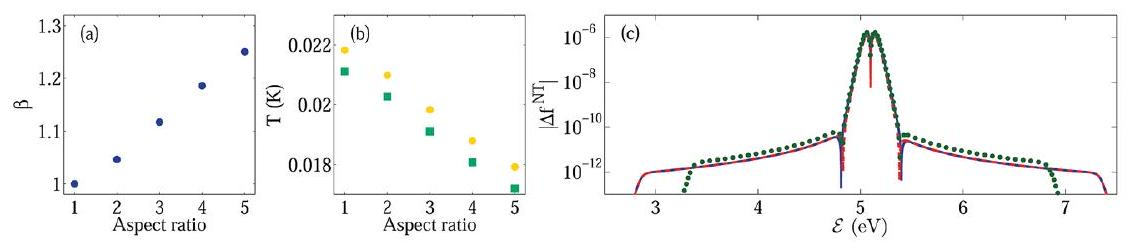
\includegraphics[alt={},max width=\textwidth]{9dd9846f-eb13-4506-8661-d691c4a998fa-07_248_1131_1623_203}
\captionsetup{labelformat=empty}
\caption{Fig. 2 (a) Geometric rescaling factor of the thermal conductivity of the host for metal nanorods with different aspect ratios. ${ }^{37}$ (b) Electron (yellow dots) and phonon (green squares) temperature rises of nanorods with different aspect ratios but identical wavelength ( 2.5 eV ), volume and averaged field ( $|\vec{E}|^{2}=10^{8}\left(\mathrm{~V} \mathrm{~m}^{-1}\right)^{2}$ ). (c) Deviation from the equilibrium distribution for the aspect ratios $1: 1$ (blue solid line) and $1: 5$ (red dashed line), respectively. The green dotted line shows the deviation from the equilibrium distribution for a different wavelength ( 1.75 eV ) with an aspect ratio of $1: 1$.}
\end{center}
\end{figure}

\section*{III. Dependence on nanoparticle size and shape}
Previous studies have claimed that particles with sharp edges, for which regions of strong electric fields (also confusingly referred to as "hot spots" ${ }^{94}$ ) of electric fields occur, are superior for the purpose of generating high energy, non-thermal carriers. Unfortunately, however, these claims were based on what we believe to be a somewhat improper comparison.

Specifically, while previous comparisons were carried out for particles of the same volume (and probably the same incident intensity), the changes in size and shape incur changes in the resonance position and quality, therefore resulting in a change in the local electric field within the NP. Thus, the differences observed in such comparisons ensue partially (if not completely) from these purely classical electromagnetic effects, meaning that it is not clear what conclusion can be made from such a comparison.

In that sense, a better suited comparison should be made for particles with the same volume and the same average internal (squared) fields, $\int_{V}|E|^{2} \mathrm{~d} V$. Such a comparison would also allow one to isolate the role of additional quantum mechanical effects from the purely classical electrodynamic considerations associated with the quality and position of the optical response. Since we observed in ref. 48 that away from the Fermi energy the density of high energy carriers is proportional to the square of the local field, $f \sim|E|^{2}$, it is immediately obvious that, to leading order, the total number of carriers at a given energy (away from the Fermi energy) is the same for NPs with the same (average) internal field, regardless of their shape and of the electric field distribution.

Some differences may still exist due to field and temperature gradients. These, however, are expected to be weak - the charge currents created by the electric field non-uniformity are assumed to be weak (due to the fast e-e collisions and the high conductance of the metal); heat currents are definitely weak - indeed, the temperature uniformity is excellent due to the high thermal conductivity within the metal. Either way, the neglect of these currents is, to the best of our knowledge, common to all previous studies, and will accordingly be adopted here as well.

Having said that, we should emphasize that the electron distribution near the Fermi energy (hence, the electron temperature) might be very sensitive to the shape and size of the NP. Indeed, the particle size and shape affect the coupling efficiency of heat to the environment, manifested via the phononenvironment coupling coefficient $G_{\text {ph-env }}$ (introduced in Section A). In ref. 37, Baffou et al. used exact numerical simulations to provide accurate empirical expressions for the effective thermal coupling coefficient to the environment for various generic particle shapes. In particular, they showed that since a spherical nanoparticle has a minimal surface area-to-volume ratio, it is optimal in terms of holding on to the heat generated within it. Accordingly, one can expect that for a given average (squared) local field (which is directly proportional to the absorbed power, see eqn (A4)), a sphere will be the hottest among all other particles. Thus, overall, while the number of non-thermal carriers generated within a sphere is the same as in any other particle (for a given average local field and particle volume), it exhibits the poorest relative efficiency of thermal vs. non-thermal energy partition.

These expectations are confirmed by numerical solutions of the Boltzmann eqn (1) for Ag rods with various aspect ratios but with the same volume. As the input electromagnetic field, we used a fixed value representing the averaged square of the local electric field rather than the field itself (see our justification above). One can see that the lowest temperature is attained for a rod with a $1: 5$ aspect ratio due to its $30 \%$ stronger coupling coefficient of heat to the environment (Fig. 2). The population of the high energy, non-thermal carriers is, however, the same for the different rods.

Our approach also shows the differences in the non-thermal distributions near the Fermi-energy for two different wavelengths. Specifically, the change in wavelength affects the shoulder width (due to the change in $\hbar \omega_{\mathrm{p}}$ ) and height (due to the change in the density of states at $\mathcal{E}$ and $p_{\text {abs }}$ with the illumination wavelength ${ }^{95}$ ). For example, $\phi_{\mathrm{A}, 1.75 \mathrm{eV}} / \phi_{\mathrm{A}, 2.25 \mathrm{eV}} \approx 1.3$ and $N_{\mathrm{A}}(1.75 \mathrm{eV}) / N_{\mathrm{A}}(2.25 \mathrm{eV})=\varepsilon_{\mathrm{m}}^{\prime \prime}(1.75 \mathrm{eV}) / \varepsilon_{\mathrm{m}}^{\prime \prime}(2.25 \mathrm{eV})=1.35$ (ref. 73) for the same average field. As a result, $\left|\Delta f_{1.75 \mathrm{eV}}^{\mathrm{NT}}\right| /\left|\Delta f_{2.25 \mathrm{eV}}^{\mathrm{NT}}\right|=\left(N_{\mathrm{A}}(1.75 \mathrm{eV}) \phi_{\mathrm{A}, 1.75 \mathrm{eV}}\right) /\left(N_{\mathrm{A}}(2.25 \mathrm{eV})\right. \left.\phi_{\mathrm{A}, 2.25 \mathrm{ev}}\right) \approx 1.76$, which is in excellent agreement with the numerical results.

\section*{IV. Non-thermal carriers and photocatalysis}
We now wish to make the connection between our theory, in which the (nonthermal) carrier distribution is evaluated, and photocatalysis, namely the enhancement of a reaction rate due to the presence of an illuminated nanoparticle ( NP ). The first stage is to understand the nature of the photocatalytic process, and its relation to the electron distribution in the NP. To this end, we follow the reasoning (based on the specific example of hydrogen molecule dissociation) presented in ref. 41, as depicted in Fig. 3. Consider a reaction pathway defined by a free energy curve in some reaction coordinate (blue solid line) leading from the initial state to the product state (in $\mathrm{H}_{2}$ dissociation the initial and product states are $H_{2} \sigma_{g}$ and the dissociated molecule 2 H , respectively,

\begin{figure}[h]
\begin{center}
  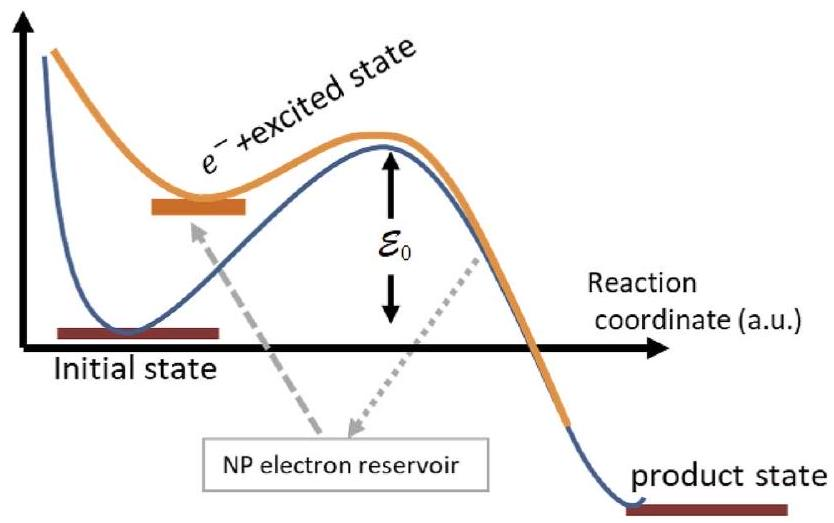
\includegraphics[alt={},max width=\textwidth]{9dd9846f-eb13-4506-8661-d691c4a998fa-09_523_834_1447_349}
\captionsetup{labelformat=empty}
\caption{Fig. 3 Schematic illustration of the photocatalytic process. The molecule absorbs an electron from the NP, thus going from the initial state to the excited state. The barrier that has to be crossed to reach the product state is much smaller now, resulting in a much higher reaction rate. During the relaxation process the excess electron returns to the NP.}
\end{center}
\end{figure}

and the reaction coordinate is the $\mathrm{H}-\mathrm{H}$ bond length). This reaction is limited by the energy barrier $\mathcal{E}_{0}\left(\sim 2.3 \mathrm{eV}\right.$ for $\mathrm{H}_{2}$ dissociation), which is practically unreachable at room temperature.

Now, the molecular system is placed in the vicinity of a NP, from which electrons with energy $\mathcal{E}_{\text {in }}$ can hop onto the molecule (dashed gray arrow), thus generating a charged excited state (the state $H_{2}^{\delta-} \sigma_{\mathrm{u}}^{*}$ in the $\mathrm{H}_{2}$ dissociation example). In this sense, the NP is nothing but an electron reservoir available to the molecular system. The excited state molecule has a different reaction path (solid orange line), with a smaller energy barrier for the reaction. This reduction of the energy barrier is the essence of the catalytic process. At some point along the reaction path, the excess electron returns to the NP with energy $\mathcal{E}_{\text {out }}$ (dotted gray arrow), and the system returns to the neutral-state reaction path. The concept of "hot electron-assisted photocatalysis" is based on the concept that illumination of the NP will dramatically increase the probability of electrons (in the NP) having energy $\mathcal{E}_{\text {in }}$, thus making their excess energy available for the chemical reaction to occur.

We can now try to relate this description to the evaluation of the electronic distribution function in the NP. For the electrons in the NP, the nearby molecule that undergoes the reaction can be considered as a source of irreversible energy loss, whereby electrons come in with energy $\mathcal{E}_{\text {in }}$ and leave, after some reaction time, $\tau_{\mathrm{r}}$, with energy $\mathcal{E}_{\text {out }}$. Therefore, within a Boltzmann equation description of the electron distribution, this term can be written as


\begin{equation*}
\left(\frac{\mathrm{d} f}{\mathrm{~d} t}\right)_{\text {react }} \sim \gamma_{\mathrm{r}} f\left(\mathcal{E}_{\text {in }}\right)\left(1-f\left(\mathcal{E}_{\text {out }}\right)\right), \tag{6}
\end{equation*}


where $\gamma_{\mathrm{r}}=\tau_{\mathrm{r}}^{-1}$ is the bare reaction rate, i.e. the rate at which the chemical system undergoes the reaction after being excited by an additional electron (which is the rate-limiting step). More realistically, one can assume that there is some broadening to the energies $\mathcal{E}_{\text {in,out }}$, resulting in a term that looks like


\begin{equation*}
\left(\frac{\mathrm{d} f}{\mathrm{~d} t}\right)_{\text {react }} \sim \gamma_{\mathrm{r}} \int \mathrm{~d} \mathcal{E} \int \mathrm{~d} \mathcal{E}^{\prime} g\left(\mathcal{E} ; \mathcal{E}_{\text {in }}, \sigma\right) g\left(\mathcal{E} ; \mathcal{E}_{\text {out }}, \sigma\right) f(\mathcal{E})\left(1-f\left(\mathcal{E}^{\prime}\right)\right), \tag{7}
\end{equation*}


where $g\left(\mathcal{E} ; \mathcal{E}_{0}, \sigma\right)$ is a Gaussian centered around $\mathcal{E}_{0}$ with width $\sigma$. Eqn (6) is reproduced if the limit $\sigma \rightarrow 0$ is taken, i.e., taking $g$ to be a $\delta$-function.

In principle, eqn (7) should be inserted into the full Boltzmann equation for the distribution function (1). However, since chemical kinetics are substantially slower than electronic processes, $\gamma_{\mathrm{r}}$ is much smaller than any of the other terms (photo-excitation, electron-electron and electron-phonon scattering terms) in the Boltzmann equation. It follows that in order to determine the steady-state distribution, the $\gamma_{\mathrm{r}}$-term can be neglected. In other words, the chemical reaction does not affect the electron distribution in the NP. The photocatalytic reaction rate is therefore defined by eqn (6) or (7), and since $1-f\left(\mathcal{E}_{\text {out }}\right) \sim 1$, it can be approximated by $\gamma_{\mathrm{r}} f\left(\mathcal{E}_{\text {in }}\right)$. This is a rather intuitive result; the photocatalytic rate is proportional to the bare reaction rate multiplied by the probability of finding an electron at the relevant energy (factors such as the density of states go into the proportionality constant). The conclusion to be drawn from this simple set of arguments is straightforward and unavoidable; if this mechanism indeed describes the experiments, then the reaction rate should increase in proportionality to the increase in the high-energy part of the electron distribution. In\\
ref. 48 as well as above (see eqn (5)), we have shown that the high-energy part of the electron distribution increases by $\sim 10$ orders of magnitude (and maybe more). This is nowhere near the increase in reaction rate observed for any experiment reporting metal NP-assisted photocatalysis; specifically, it is far higher than what was observed in ref. 74, which found a mild 6-fold increase in the reaction rate. We therefore conclude that "hot carriers" are extremely unlikely to be responsible for the observed increase in the reaction rate. The strong dependence of the photocatalytic rate on the substrate implies that the reason for the faster chemistry is merely heating. Indeed, faster reactions were observed with a glass substrate, which has a much lower thermal conductivity (in comparison with the $\mathrm{TiO}_{2}$ substrate used in ref. 41), thus giving rise to higher temperatures in the nanoparticles.

\section*{V. Summary \& outlook}
The simplified analysis of Section II enables an effortless determination of the electron distribution function, the electron temperature and the phonon temperature for metals under steady-state illumination. This should motivate a re-examination of all previous recent theoretical studies of the nonequilibrium in metallic nanostructures that did not account for thermal effects. It should also be the basis for improved modelling, e.g. by accounting for more realistic band structures (thus enabling a comparison of different metals), considering more complex nanostructures (involving different materials, especially semiconductors that provide an independent source of "hot" carriers ${ }^{42}$ ), adding (secondary) physical mechanisms (surface states, carrier tunneling, field and temperature gradients etc.), and studying the competing contributions of thermal and non-thermal effects to the nonlinear response of metals etc.

Our results also enable a re-evaluation of the interpretations of previous experiments. In particular, since the model reported in Section IV predicts dramatically faster chemistry (many orders of magnitude faster reaction rates), the absence of such an effect in the experimental data reported thus far implies that it is extremely unlikely that the faster chemistry reported was indeed due to the generation of high energy, non-thermal carriers. This conclusion should induce a more careful examination of the origin and energy scale of the faster reactions in those studies, which are far less sensitive to the presence of the metal and illumination than predicted in Section IV. Most likely, the mechanism responsible for the faster reactions will turn out to be mere regular heating. Conversely, our theory can provide insight into the design of experiments in which high energy, non-thermal carriers are dominant.

In this vein, we hope that our results will motivate a quantitative comparison of the theoretical predictions with experimental data. The latter should include measurements of the metal temperature using one of the emerging techniques (e.g., ref. 34-36, 75-80) together with electron photo-emission spectroscopy measurements. ${ }^{\mathbf{8 1 - 8 3}}$ Ideally, these measurements should be carried out for a single particle (such as in ref. $42,81,84$ and 85 ) in order to exclude multi-particle heating interactions, which are relatively hard to quantify. ${ }^{\mathbf{4 0 , 4 1}}$

\section*{Appendix: A. An estimate of the quantum mechanical excitation term for CW illumination of a metal nanoparticle}
We employ the elegant expression proposed in ref. 57; namely, we define $A(\mathcal{E} ; \omega)$ such that $A(\mathcal{E} ; \omega) \mathrm{d} \omega \mathrm{d} \mathcal{E}$ is the (joint) probability of photon absorption of frequency between $\omega$ and $\omega+\mathrm{d} \omega$ for the final energy $\mathcal{E}$ measured with respect to the bottom of the band at $\mathcal{E}=0$. We define this probability as


\begin{equation*}
A\left(\mathcal{E}_{\text {final }}=\mathcal{E} ; \omega\right)=\frac{n_{\mathrm{A}}(\omega)}{N_{\mathrm{A}}} \frac{D_{\mathrm{J}}(\mathcal{E}, \mathcal{E}-\hbar \omega) \rho_{\mathrm{J}}(\mathcal{E}, \mathcal{E}-\hbar \omega)}{\int D_{\mathrm{E}}(\mathcal{E}, \mathcal{E}-\hbar \omega) \rho_{\mathrm{J}}(\mathcal{E}, \mathcal{E}-\hbar \omega) \mathrm{d} \mathcal{E}}, \tag{A1}
\end{equation*}


where $D_{\mathrm{J}}\left(\mathcal{E}_{\text {final }}, \mathcal{E}_{\text {initial }}\right)$ is the squared magnitude of a transition matrix element for the electronic process $\mathcal{E}_{\text {initial }} \rightarrow \mathcal{E}_{\text {final }}$. Furthermore, $\rho_{\mathrm{J}}$ corresponds to the population-weighted density of pair states,


\begin{equation*}
\rho_{\mathrm{J}}\left(\mathcal{E}_{\text {final }}, \mathcal{E}_{\text {initial }}\right)=\left[f\left(\mathcal{E}_{\text {initial }}\right) \rho_{\mathrm{e}}\left(\mathcal{E}_{\text {initial }}\right)\right]\left[1-f\left(\mathcal{E}_{\text {final }}\right) \rho_{\mathrm{e}}\left(\mathcal{E}_{\text {final }}\right)\right] \tag{A2}
\end{equation*}


and $\rho_{\mathrm{e}}=\frac{3 n_{\mathrm{e}}}{2 \mathcal{E}_{\mathrm{F}}} \sqrt{\frac{\mathcal{E}}{\mathcal{E}_{\mathrm{F}}}}$ is the density of states of a free electron gas; ${ }^{\text {50 }} n_{\mathrm{e}}$ is the electron density. Finally, $n_{\mathrm{A}}(\omega)$ is the number density of absorbed $\hbar \omega$ photons per unit time between $\omega$ and $\omega+\mathrm{d} \omega$, and $N_{\mathrm{A}}=\int \mathrm{d} \omega n_{\mathrm{A}}(\omega)$ is the total number density of absorbed photons per unit time. For CW illumination, this is given by


\begin{equation*}
N_{\mathrm{A}}=\frac{\left\langle p_{\mathrm{abs}}\right\rangle}{\hbar \omega}, \tag{A3}
\end{equation*}


where the averaged absorbed optical power density (in units of $\mathrm{W} \mathrm{m}^{-3}$ ) is given by the Poynting vector, ${ }^{86}$ namely


\begin{equation*}
\left\langle p_{\mathrm{abs}}\right\rangle=\omega \varepsilon^{\prime \prime}\left(\omega, T_{\mathrm{e}}, T_{\mathrm{ph}}\right)\langle\vec{E}(\vec{r}, t) \cdot \vec{E}(\vec{r}, t)\rangle_{t, \vec{r}} \tag{A4}
\end{equation*}


where $\varepsilon^{\prime \prime}$ is the imaginary part of the metal permittivity, and the spatio-temporal averaging, $\rangle t, \vec{r}$, is performed over a single optical cycle such that only the timeindependent component remains and is over the NP volume.

The net change of electronic population at energy $\mathcal{E}$ per unit time and energy at time $t$ due to absorption is $N_{\mathrm{A}} \phi_{\mathrm{A}}$, where


\begin{equation*}
\phi_{\mathrm{A}}(\mathcal{E} ; \omega)=\int_{0}^{\infty} \mathrm{d} \omega[A(\mathcal{E} ; \omega)-A(\mathcal{E}+\hbar \omega ; \omega)] \tag{A5}
\end{equation*}


describes the total (probability of a) population change at energy $\mathcal{E}$ per unit time and energy at time $t$. Altogether,


\begin{equation*}
\left(\frac{\partial f}{\partial t}\right)_{\mathrm{ex}}=\frac{N_{\mathrm{A}} \phi_{\mathrm{A}}(E)}{\rho_{\mathrm{e}}(E)} \tag{A6}
\end{equation*}


meaning that electron number conservation is ensured, $\int \mathrm{d} \mathcal{E} \rho_{\mathrm{e}}(\mathcal{E})(\partial f / \partial \mathcal{E})_{\mathrm{ex}} \sim \int \mathrm{d} \mathcal{E} \phi_{\mathrm{A}}(\mathcal{E})=0$.

For CW illumination, $n_{\mathrm{A}}=N_{\mathrm{A}} \delta\left(\omega-\omega_{\mathrm{p}}\right)$ and $N_{\mathrm{A}}=2 \varepsilon_{\mathrm{m}}^{\prime \prime}\left(\omega_{\mathrm{p}}, T_{\mathrm{e}}, T_{\mathrm{ph}}\right)\left|E\left(\omega_{\mathrm{p}}\right)\right|^{2} / \hbar$. For the low intensities considered here, one can ignore the temperature dependence of the metal permittivity. ${ }^{38,87}$

\begin{table}[h]
\begin{center}
\captionsetup{labelformat=empty}
\caption{Table 1 Parameters used in the simulations and the values chosen for (low quality) ${ }^{73} \mathrm{Ag}$}
\begin{tabular}{|l|l|l|}
\hline
Parameter & Parameter symbol & Value \\
\hline
Photon wavelength & $\lambda$ & 2.25 eV \\
\hline
Metal permittivity & $\varepsilon_{\text {Ag }}(\lambda)$ & $-8.5+1.8 i^{73}$ \\
\hline
Fermi energy & $\mathcal{E}_{\mathrm{F}}$ & 5.1 eV \\
\hline
Conduction band width & $\mathcal{E}_{\text {max }}$ & 9 eV \\
\hline
Chemical potential & $\mu$ & 5.1 eV \\
\hline
Electron density & $n_{\mathrm{e}}$ & $5.86 \times 10^{28} \mathrm{~m}^{-3}$ \\
\hline
Ambient temperature & $T_{\text {amb }}$ & 297 K \\
\hline
Electron mass & $m_{\mathrm{e}}$ & $9.1 \times 10^{31} \mathrm{~kg}$ \\
\hline
\end{tabular}
\end{center}
\end{table}

For simplicity, we now approximate $\rho_{\mathrm{e}}$ by its value at $\mathcal{E}_{\mathrm{F}}$. In the same spirit, we define the normalized transition matrix element $\bar{D} \equiv \int D_{\mathrm{J}}\left(E, E-\hbar \omega_{\mathrm{p}}\right) \rho_{\mathrm{J}}\left(E, E-\hbar \omega_{\mathrm{p}}\right) \mathrm{d} E / D_{\mathrm{J}}\left(E, E-\hbar \omega_{\mathrm{p}}\right)$ and ignore its energydependence. Thus, we also find that $\bar{D} \cong \int D_{\mathrm{J}}\left(E+\hbar \omega_{\mathrm{p}}, E\right) \rho_{\mathrm{J}}\left(E+\hbar \omega_{\mathrm{p}}, E\right) \mathrm{d} E / D_{\mathrm{J}}\left(E+\hbar \omega_{\mathrm{p}}, E\right)$, meaning that $\bar{D} \approx \int \rho_{\mathrm{J}} \mathrm{d} E \approx \rho_{\mathrm{e}}{ }^{2}\left(E_{\mathrm{F}}\right) / E_{\text {max }}$. In this case, the excitation rate (A6) can be approximated by


\begin{equation*}
\left(\frac{\partial f}{\partial t}\right)_{\mathrm{ex}}=\frac{N_{\mathrm{A}}}{\bar{D}} \rho_{\mathrm{e}}\left(E_{\mathrm{F}}\right) B(E)=\frac{2 \varepsilon_{\mathrm{m}}^{\prime \prime}}{\hbar} \frac{B(E)|E|^{2}}{E_{\max } \rho_{\mathrm{e}}\left(E_{\mathrm{F}}\right)}=\mathrm{RB}(E)|E|^{2}, \tag{A7}
\end{equation*}


where $B(\mathcal{E})=f\left(\mathcal{E}-\hbar \omega_{\mathrm{p}}\right)(1-f(\mathcal{E}))-f(\mathcal{E})\left(1-f\left(\mathcal{E}+\hbar \omega_{\mathrm{p}}\right)\right)$ is a dimensionless $\mathrm{O}(1)$ function representing the $2 \hbar \omega_{\mathrm{p}}$ step-like energy dependence of the quantum excitation term and $R \equiv \frac{4 \varepsilon_{0} \varepsilon_{\mathrm{m}}^{\prime \prime}\left(\omega_{\mathrm{p}}\right)}{3 \hbar n_{\mathrm{e}}} \frac{E_{\mathrm{F}}}{E_{\text {max }}} \approx 2 \times 10^{-6} \mathrm{~m}^{2} \mathrm{~V}^{-2} \mathrm{~s}^{-1}$ (see the parameter definitions and values in Table 1). Thus, we can estimate the non-thermal carrier density as


\begin{equation*}
\Delta f \equiv f-f^{T}\left(E, T_{\mathrm{env}}\right) \approx \tau_{\mathrm{e}-\mathrm{e}} R|E|^{2}=4 \times 10^{-20}|E|^{2}\left[\mathrm{~V}^{2} \mathrm{~m}^{-2}\right] . \tag{A8}
\end{equation*}


\section*{Conflicts of interest}
There are no conflicts to declare.

\section*{References}
1 A. O. Govorov and H. H. Richardson, Generating heat with metal nanoparticles, Nano Today, 2007, 2, 30-38.\\
2 G. Baffou and R. Quidant, Thermo-plasmonics: using metallic nanostructures as nano-sources of heat, Laser Photonics Rev., 2013, 7, 171-187.\\
3 D. Boyer, P. Tamarat, A. Maali, B. Lounis and M. Orrit, Photothermal imaging of nanometer-sized metal particles among scatterers, Science, 2002, 297, 11601163.

4 V. P. Zharov and D. O. Lapotko, Photothermal imaging of nanoparticles and cells, IEEE J. Sel. Top. Quantum Electron., 2005, 11, 733-751.

5 M. W. Dewhirst, B. L. Viglianti, M. Lora-Michiels, M. Hanson and P. J. Hoopes, Basic principles of thermal dosimetry and thermal thresholds for tissue damage from hyperthermia, Int. J. Hyperthermia, 2003, 19, 267-294.

6 H. A. Atwater and A. Polman, Plasmonics for improved photovoltaic devices, Nat. Mater., 2010, 9, 205-213.\\
7 G. Baffou, J. Polleux, H. Rigneault and S. Monneret, Super-heating and microbubble generation around plasmonic nanoparticles under CW illumination, $J$. Phys. Chem. C, 2014, 118, 4890-4898.\\
8 O. Neumann, A. S. Urban, J. Day, S. Lal, P. Nordlander and N. J. Halas, Solar vapor generation enabled by nanoparticles, ACS Nano, 2013, 7, 42-49.\\
9 Z. Fang, Y. R. Zhen, O. Neumann, A. Polman, F. J. Garcia de Abajo, P. Nordlander and N. J. Halas, Evolution of light-induced vapor generation at a liquid-immersed metallic nanoparticle, Nano Lett., 2013, 13, 1736-1742.\\
10 H. M. L. Robert, F. Kundrat, E. Bermúdez-Ure na, H. Rigneault, S. Monneret, R. Quidant, J. Polleux and G. Baffou, Light-assisted solvothermal chemistry using plasmonic nanoparticles, ACS Omega, 2016, 1, 2-8.\\
11 S. Molesky, C. J. Dewalt and Z. Jacob, High temperature epsilon-near-zero and epsilon-near-pole metamaterial emitters for thermophotovoltaics, Opt. Express, 20113, 21, A96-A110.\\
12 J. Liu, U. Guler, A. Lagutchev, A. V. Kildishev, O. Malis, A. Boltasseva and V. M. Shalaev, Quasi-coherent thermal emitter based on refractory plasmonic materials, Opt. Mater. Express, 2014, 5, 2721-2728.\\
13 J. B. Khurgin, G. Sun, W. T. Chen, W.-Y. Tsai and D. P. Tsai, Ultrafast thermal nonlinearity, Sci. Rep., 2015, 5, 17899.\\
14 E. Rousseau, A. Siria, G. Jourdan, S. Volz, F. Comin, J. Chevrier and J.-J. Greffet, Radiative heat transfer at the nanoscale, Nat. Photonics, 2009, 3, 514-517.\\
15 D. A. Boyd, L. Greengard, M. Brongersma, M. Y. El-Naggar and D. G. Goodwin, Plasmon-assisted chemical vapor deposition, Nano Lett., 2006, 6, 2592-2597.\\
16 U. Guler, A. Boltasseva and V. M. Shalaev, Refractory plasmonics, Science, 2014, 334, 263.\\
17 K. Watanabe, D. Menzel, N. Nilius and H.-J. Freund, Photochemistry on metal nanoparticles, Chem. Rev., 2006, 106, 4301-4320.\\
18 A. Naldoni, F. Riboni, U. Guler, A. Boltasseva, V. M. Shalaev and A. V. Kildishev, Solar-powered plasmon-enhanced heterogeneous catalysis, Nanophotonics, 2016, 5, 112-133.\\
19 S. Linic, P. Christopher and D. B. Ingram, Plasmonic-metal nanostructures for efficient conversion of solar to chemical energy, Nat. Mater., 2011, 10, 911-921.\\
20 C. Clavero, Plasmon-induced hot-electron generation at nanoparticle/metaloxide interfaces for photovoltaic and photocatalytic devices, Nat. Photonics, 2014, 8, 95-103.\\
21 G. Baffou and R. Quidant, Nanoplasmonics for chemistry, Chem. Soc. Rev., 2014, 43, 3898.\\
22 M. L. Brongersma, N. J. Halas and P. Nordlander, Plasmon-induced hot carrier science and technology, Nat. Nanotechnol., 2015, 10, 25.\\
23 M. Moskovits, The case for plasmon-derived hot carrier devices, Nat. Nanotechnol., 2015, 10, 6.\\
24 S. Mubeen, J. Lee, N. Singh, S. Kraemer, G. D. Stucky and M. Moskovits, An autonomous photosynthetic device in which all charge carriers derive from surface plasmons, Nat. Nanotechnol., 2013, 8, 247-251.

25 K. Ueno, T. Oshikiri, X. Shi, Y. Zhong and H. Misawa, Plasmon-induced artificial photosynthesis, Interface Focus, 2014, 5, 20140082.\\
26 I. Goykhman, B. Desiatov, J. Khurgin, J. Shappir and U. Levy, Locally oxidized silicon surface-plasmon Schottky detector for telecom regime, Nano Lett., 2011, 11, 2219-2224.\\
27 I. Goykhman, B. Desiatov, J. Khurgin, J. Shappir and U. Levy, Waveguide based compact silicon Schottky photodetector with enhanced responsivity in the telecom spectral band, Opt. Express, 2012, 20, 28594.\\
28 M. W. Knight, Y. Wang, A. S. Urban, A. Sobhani, B. Y. Zheng, P. Nordlander and N. J. Halas, Embedding plasmonic nanostructure diodes enhances hot electron emission, Nano Lett., 2013, 13, 1687-1692.\\
29 W. Li and J. Valentine, Harvesting the loss: Surface plasmon-based hot electron photodetection, Nanophotonics, 2016, 6, 177-191.\\
30 A. Giugni, B. Torre, A. Toma, M. Francardi, M. Malerba, A. Alabastri, R. Proietti Zaccaria, M. I. Stockman and E. Di Fabrizio, Hot-electron nanoscopy using adiabatic compression of surface plasmons, Nat. Nanotechnol., 2013, 8, 845852.

31 G. V. Naik and J. A. Dionne, Photon upconversion with hot carriers in plasmonic systems, Appl. Phys. Lett., 2015, 107, 133902.\\
32 G. V. Naik, A. J. Welch, J. A. Briggs, M. L. Solomon and J. A. Dionne, Hot-carrier-mediated photon upconversion in metal-decorated quantum wells, Nano Lett., 2017, 17, 4583-4587.\\
33 X. Zhou, G. Liu, J. Yu and W. Fan, Surface plasmon resonance-mediated photocatalysis by noble metal-based composites under visible light, J. Mater. Chem., 2012, 22, 21337-21354.\\
34 J. T. Hugall and J. J. Baumberg, Demonstrating photoluminescence from Au is electronic inelastic light scattering of a plasmonic metal: The origin of SERS backgrounds, Nano Lett., 2015, 15, 2600-2604.\\
35 X. Xie and D. G. Cahill, Gold nanoparticles as absolute nano-thermometers, Appl. Phys. Lett., 2016, 109, 183104.\\
36 A. Carattino, M. Caldarola and M. Orrit, Gold nanoparticles as absolute nanothermometers, Nano Lett., 2017, 18, 874-880.\\
37 G. Baffou, R. Quidant and F. J. Garcia de Abajo, Nanoscale control of optical heating in complex plasmonic systems, ACS Nano, 2010, 4, 709-716.\\
38 Y. Sivan and S.-W. Chu, Nonlinear plasmonics at high temperatures, Nanophotonics, 2017, 6, 317-328.\\
39 H. H. Richardson, M. T. Carlson, P. J. Tandler, P. Hernandez and A. O. Govorov, Experimental and theoretical studiesof light-to-heat conversion and collective heating effects in metal nanoparticle solutions, Nano Lett., 2009, 9, 1139-1146.\\
40 G. Baffou, P. Berto, E. Bermudez Urena, R. Quidant, S. Monneret, J. Polleux and H. Rigneault, Photoinduced heating of nanoparticle arrays, ACS Nano, 2013, 7, 6478-6488.\\
41 S. Mukherjee, L. Zhou, A. Goodman, N. Large, C. Ayala-Orozco, Y. Zhang, P. Nordlander and N. J. Halas, Hot-electron-induced dissociation of H 2 on gold nanoparticles supported on SiO2, J. Am. Chem. Soc., 2014, 136, 64-67.\\
42 S. Tan, A. Argondizzo, J. Ren, L. Liu, J. Zhao and H. Petek, Plasmonic coupling at a metal/semiconductor interface, Nat. Photonics, 2017, 11, 806-812.

43 L. Zhou, D. F. Swearer, C. Zhang, H. Robatjazi, H. Zhao, L. Henderson, L. Dong, P. Christopher, E. A. Carter, P. Nordlander and N. J. Halas, Quantifying hot carrier and thermal contributions in plasmonic photocatalysis, Science, 2018, 362, 69.\\
44 X. Zhang, X. Li, M. E. Reish, D. Zhang, N. Q. Su, Y. Gutiërrez, F. Moreno, W. Yang, H. O. Everitt and J. Liu, Plasmon-enhanced catalysis: Distinguishing thermal and nonthermal effects, Nano Lett., 2018, 18, 17141723.

45 A. Puglisi, A. Sarracino and A. Vulpiani, Temperature in and out of equilibrium: a review of concepts, tools and attempts, Phys. Rep., 2017, 709710, 1-60.\\
46 L. D. Pietanza, G. Colonna, S. Longo and M. Capitelli, Non-equilibrium electron and phonon dynamics in metals under femtosecond laser pulses, Eur. Phys. J. D, 2007, 45, 369-389.\\
47 J. R. M. Saavedra, A. Asenjo-Garcia and F. Javier Garcia de Abajo, Hot-electron dynamics and thermalization in small metallic nanoparticles, ACS Photonics, 2016, 3, 1637-1646.\\
48 Y. Dubi and Y. Sivan, "Hot electrons" in metallic nanostructures - non-thermal carriers or heating?, Nat. Photonics, 2018, under review.\\
49 J. M. Ziman, Principles of the theory of solids. Cambridge University Press, 1972.

50 N. W. Ashcroft and N. D. Mermin, Solid state physics, Brooks/Cole, 1976.\\
51 D. Pines and P. Nozieres, The theory of quantum liquids, Benjamin, New York, 1966.

52 M. Dressel and G. Grüner, Electrodynamics of solids - optical properties of electrons in matter, Cambridge University Press, 2002.\\
53 R. H. M. Groeneveld, R. Sprik and A. Lagendijk, Femtosecond spectroscopy of electron-electron and electron-phonon energy relaxation in Ag and Au, Phys. Rev. B: Condens. Matter Mater. Phys., 1995, 51, 11433-11445.\\
54 N. Del Fatti, C. Voisin, M. Achermann, S. Tzortzakis, D. Christofilos and F. Valleé, Nonequilibrium electron dynamics in noble metals, Phys. Rev. B: Condens. Matter Mater. Phys., 2000, 61, 16956-16966.\\
55 B. Rethfeld, A. Kaiser, M. Vicanek and G. Simon, Ultrafast dynamics of nonequilibrium electrons in metals under femtosecond laser irradiation, Phys. Rev. B: Condens. Matter Mater. Phys., 2002, 65, 214303.\\
56 P. Grua, J. P. Morreeuw, H. Bercegol, G. Jonusauskas and F. Valleé, Electron kinetics and emission for metal nanoparticles exposed to intense laser pulses, Phys. Rev. B: Condens. Matter Mater. Phys., 2003, 68, 035424.\\
57 M. Kornbluth, A. Nitzan and T. Seidman, Light-induced electronic nonequilibrium in plasmonic particles, J. Chem. Phys., 2013, 138, 174707.\\
58 R. W. Schoenlein, W. Z. Lin, J. G. Fujimoto and G. L. Eesley, Femtosecond studies of nonequilibrium electronic processes in metals, Phys. Rev. Lett., 1987, 58, 1680-1683.\\
59 E. Carpene, Ultrafast laser irradiation of metals: Beyond the two-temperature model, Phys. Rev. B: Condens. Matter Mater. Phys., 2006, 74, 024301.\\
60 G. Della Valle, M. Conforti, S. Longhi, G. Cerullo and D. Brida, Real-time optical mapping of the dynamics of nonthermal electrons in thin gold films, Phys. Rev. B: Condens. Matter Mater. Phys., 2012, 86, 155139.

61 P. E. Hopkins, Contributions of inter and intra-band excitations to electron heat capacity and electron-phonon coupling in noble metals, J. Heat Transfer, 2010, 132, 014504.

62 A. Giri and P. E. Hopkins, Transient thermal and nonthermal electron and phonon relaxation after short-pulsed laser heating of metals, J. Appl. Physiol., 2015, 118, 215101.\\
63 A. M. Brown, R. Sundararaman, P. Narang, W. A. Goddard and H. A. Atwater, Ab initio phonon coupling and optical response of hot electrons in plasmonic metals, Phys. Rev. B, 2016, 94, 075120.\\
64 J. K. Chen, D. Y. Tzou and J. E. Beraun, A semiclassical two-temperature model for ultrafast laser heating, Int. J. Heat Mass Transfer, 2006, 49, 307-316.\\
65 V. V. Baranov and V. V. Kabanov, Theory of the electron relaxation in metals excited by an ultrashort optical pump, Phys. Rev. B: Condens. Matter Mater. Phys., 2014, 84, 125102.\\
66 J. Zhou, N. Li and R. Yang, An electrohydrodynamics model for nonequilibrium electron and phonon transport in metal films after ultra-short pulse laser heating, Eur. Phys. J. B, 2015, 88, 156.\\
67 A. Manjavacas, J. G. Liu, V. Kulkarni and P. Nordlander, Plasmon-induced hot carriers in metallic nanoparticles, ACS Nano, 2014, 8, 7630-7638.\\
68 L. V. Besteiro, X.-T. Kong, Z. Wang, G. Hartland and A. O. Govorov, Understanding hot-electron generation and plasmon relaxation in metal nanocrystals: Quantum and classical mechanisms, ACS Photonics, 2017, 4, 2759-2781.\\
69 T. Gong and J. N. Munday, Materials for hot carrier plasmonics, Opt. Mater. Express, 2015, 5, 2501.\\
70 S. Dal Forno, L. Ranno and J. Lischner, Material, size and environment dependence of plasmon-induced hot carriers in metallic nanoparticles, $J$. Phys. Chem. C, 2018, 122, 8517-8527.\\
71 J. Zhao, S. C. Nguyen, R. Ye, B. Ye, H. Weller, G. A. Somorjai, A. P. Alivisatos and F. D. Toste, A comparison of photocatalytic activities of gold nanoparticles following plasmonic and interband excitation and a strategy for harnessing interband hot carriers for solution phase photocatalysis, ACS Cent. Sci., 2017, 3, 482.\\
72 A. M. Brown, R. Sundararaman, P. Narang, W. A. Goddard and H. A. Atwater, Nonradiative plasmon decay and hot carrier dynamics: Effects of phonons, surfaces, and geometry, ACS Nano, 2016, 10, 957-966.\\
73 S. T. Sundari, S. Chandra and A. K. Tyagi, Temperature dependent optical properties of silver from spectroscopic ellipsometry and density functional theory calculations, J. Appl. Phys., 033515, 114, 2013.\\
74 S. Mukherjee, F. Libisch, N. Large, O. Neumann, L. V. Brown, J. Cheng, J. Britt Lassiter, E. A. Carter, P. Nordlander and N. J. Halas, Hot electrons do the impossible: Plasmon-induced dissociation of H2 on Au, Nano Lett., 2013, 13, 240-247.\\
75 M. Honda, Y. Saito, N. I. Smith, K. Fujita and S. Kawata, Nanoscale heating of laser irradiated single gold nanoparticles in liquid, Opt. Express, 2011, 19, 12375-12383.\\
76 M. Mecklenburg, W. A. Hubbard, E. R. White, R. Dhall, S. B. Cronin, S. Aloni and B. C. Regan, Nanoscale temperature mapping in operating microelectronic devices, Science, 2015, 347, 629.

77 G. Kucsko, P. C. Maurer, N. Y. Yao, M. Kubo, H. J. Noh, P. K. Lo, H. Park and M. D. Lukin, Nanometre-scale thermometry in a living cell, Nature, 2013, 500, 54-58.

78 S. Sadat, A. Tan, Y. J. Chua and P. Reddy, Nanoscale thermometry using point contact thermocouples, Nano Lett., 2010, 10, 2613-2617.\\
79 K. Kim, B. Song, V. Fernández-Hurtado, W. Lee, W. Jeong, L. Cui, D. Thompson, J. Feist, M. T. Homer Reid, F. J. García-Vidal, J. Carlos Cuevas, E. Meyhofer and P. Reddy, Radiative heat transfer in the extreme near field, Nature, 2015, 528, 387-391.\\
80 Y.-K. Tzeng, P.-C. Tsai, H.-Y. Liu, O. Y. Chen, H. Hsu, F.-G. Yee, M.-S. Chang and H.-C. Chang, Time-resolved luminescence nanothermometry with nitrogen-vacancy centers in nanodiamonds, Nano Lett., 2015, 15, 3945-3952.\\
81 M. Lisowski, A. P. Loukakos, U. Bovensiepen, J. Stähler, C. Gahl and M. Wolf, Ultra-fast dynamics of electron thermalization, cooling and transport effects in Ru(001), Appl. Phys. A, 2004, 78, 165-176.\\
82 M. Bauer, A. Marienfeld and M. Aeschlimann, Hot electron lifetimes in metals probed by time-resolved two-photon photoemission, Prog. Surf. Sci., 2015, 90, 319-376.\\
83 J. Vogelsang, J. Robin, B. J. Nagy, P. Dombi, D. Rosenkranz, M. Schiek, P. Gross and C. Lienau, Ultrafast electron emission from a sharp metal nanotaper driven by adiabatic nanofocusing of surface plasmons, Nano Lett., 2015, 15, 4685-4691.\\
84 Y. Levartovsky and E. Gross, High spatial resolution mapping of chemicallyactive self-assembled n-heterocyclic carbenes on Pt nanoparticles, Faraday Discuss., 2016, 5188, 345.\\
85 C.-Y. Wu, W. J. Wolf, Y. Levartovsky, H. A. Bechtel, M. C. Martin, F. D. Toste and E. Gross, High-spatial-resolution mapping of catalytic reactions on single particles, Nature, 2017, 541, 511-515.\\
86 J. D. Jackson, Classical electrodynamics, Wiley \& Sons, 3rd edn, 1998.\\
87 I. Gurwich and Y. Sivan, A metal nanosphere under intense continuous wave illumination - a unique case of non-perturbative nonlinear nanophotonics, Phys. Rev. E, 2017, 96, 012212.\\
88 Negative values of $f-f^{\mathrm{T}}$ are referred to as holes, regardless of their position with respect to the Fermi energy. This nomenclature is conventional within the literature ${ }^{51}$\\
89 Note that we ignore here the difference between the Fermi energy and the chemical potential; we verified via simulations that the difference between them is truly negligible in all of the cases we studied.\\
90 Note that the eTTM does not capture the increase in the rate of energy transfer to the lattice during the thermalization time, as discussed in ref. 53. However, this effect should have, at most, a modest quantitative effect on the issues discussed in the current work.\\
91 Note that the differences between eqn (A) and the more conventional TTM extend only to the initial non-thermal regime, for which the temperature is anyhow not well defined.\\
92 Yet, in these papers, the authors did not attempt to claim more than a qualitative prediction of the "hot electron" density.\\
$93 Z$ being the material impedance of the gas/semiconductor and $n$ its refractive index.

94 Indeed, due to the high thermal conductivity of the metal, the temperature itself is uniform across the NPs, meaning that the "hot" spot is not hotter than other regions.

95 In principle, the matrix element may also change with wavelength. However, this effect is not taken into account in the current calculation.


\end{document}